\documentclass[document.tex]{subfiles}
\begin{document}
\section*{Exercise 3:}

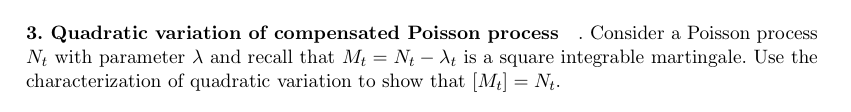
\includegraphics[width=\textwidth]{ex3.png}
\begin{equation}
Z_t = exp(M_t - \frac{1}{2} [M]_t)
\end{equation}

We use Ito's formula
\begin{equation}
M_t - \frac{1}{2} [M]_t = ln(Z_0) + \int_0^t \frac{1}{Z_s} d Z_s - \frac{1}{2} \int_0^t \frac{1}{(Z_s)^2} d [Z]_s
\end{equation}
\begin{equation}
M_t - \frac{1}{2} [M]_t = ln(Z_0) + ln(Z_t) - ln(Z_0) - \frac{1}{2} [\int_0^. \frac{1}{Z_s} d Z_s]_t
\end{equation}
\begin{equation}
M_t - \frac{1}{2} [M]_t = ln(Z_t) - \frac{1}{2} [ln(Z)]_t
\end{equation}

From this we conclude that one solution is $M_t = ln(Z_t)$.



\end{document}
